\section{基于ZMP的双足(人形)机器人行走轨迹生成}
    \subsection{基本的ZMP原理}
        ZMP(zero moment point)基于倒立摆模型提出,原理是通过让机器人与外界的作用力所
        在作用线通过虚拟的ZMP点$\boldsymbol{x}_{ZMP}$与机器人质心$\boldsymbol{x}_G$,该作用力不对机器人产生力矩
        ,同时该作用力与$\boldsymbol{x}_{G}-\boldsymbol{x}_{ZMP}$成正比\cite{sugiharaRealtimeHumanoidMotion2002},
        原理如图\ref{fig1-1}所示,其动力学方程为式\eqref{equ1-1}。
        \begin{figure}[h] %figure浮动体
            \centering
            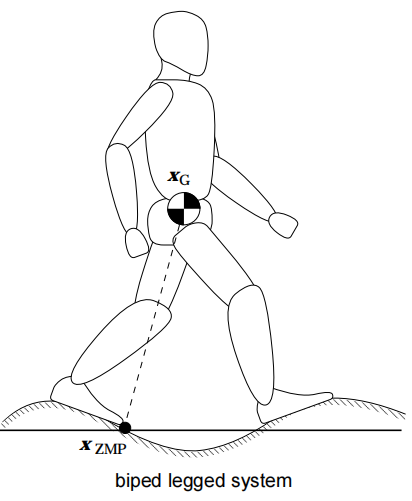
\includegraphics[scale=0.5]{2021-08-14-14-05-50.png}
            \caption{ZMP原理示意图} \label{fig1-1}
        \end{figure}
        \begin{equation}
            \begin{cases}
            m\boldsymbol{\ddot{x}}_G=-m\boldsymbol{g}+\boldsymbol{f}\\
            \boldsymbol{f}=k\left( \boldsymbol{x}_G-\boldsymbol{x}_{ZMP} \right)\\
            \end{cases} \label{equ1-1}
        \end{equation}

        在$\boldsymbol{\ddot{x}}_G$各个分量中限制分量$\ddot{z}_G$(可通过控制方法使其收敛到0)
        则其余分量可表示为式\eqref{equ1-2},实际ZMP位置的控制则可通过设定一个参考的ZMP位置值代入该式进行控制。
        \begin{equation}
            \boldsymbol{\ddot{x}}_{G,xy}=\frac{\ddot{z}_G+g}{z_G-z_{ZMP}}\left( \boldsymbol{x}_{G,xy}-\boldsymbol{x}_{ZMP,xy} \right) 
            \label{equ1-2}
        \end{equation}
    \subsection{支撑多边形(support polygon)与VHP(Virtual Horizontal Plane)的定义}
        支撑多边形可用于检测ZMP的合理位置区间,构建VHP通过ZMP点(即$z_{VHP}=z_{ZMP}$),机器人与环境的接触点${\boldsymbol{P}_1}\sim{\boldsymbol{P}_N}$与$\boldsymbol{x}_G$
        的连线交VHP于点${\boldsymbol{P}_1}^{'}\sim{\boldsymbol{P}_N}^{'}$以这些点作凸包(convex hull)得到VHP面上撑多边形,如图\ref{fig1-2}所示。
        \begin{figure}[h] %figure浮动体
            \centering
            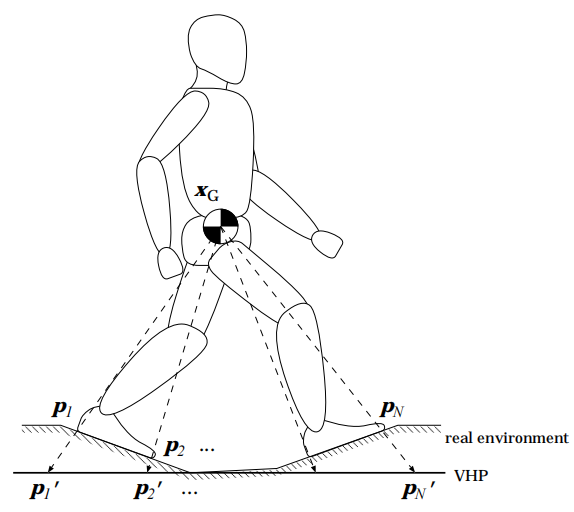
\includegraphics[scale=0.5]{2021-08-16-22-34-22.png}
            \caption{支撑多边形与VHP示意图} \label{fig1-2}
        \end{figure}
        